\chapter{Software Integration}\label{chap:integration}

This section provides an overview on how the developed pre-processing tools and \gls{ML}/\gls{DL} models were integrated in \textit{ProPythia} and \textit{OmniumAI} software platforms.

\section{ProPythia}

As mentioned in Section~\ref{sec:context_and_motivation}, \textit{ProPythia}~\cite{Sequeira2020ProPythia:Learning} is a platform devoted to the classification of peptide/protein sequences using \gls{ML} and \gls{DL}, developed within the Biosystems group at CEB/ U. Minho. Included in \textit{ProPythia} are modules to read and modify sequences, calculate various types of protein descriptors, pre-process datasets, execute feature selection and dimensionality reduction, visualize t-SNE and UMAP, perform clustering, train and optimize \gls{ML} and \gls{DL} models, and make predictions using various algorithms. \textit{ProPythia} features an adjustable modular design that makes it a flexible and user-friendly tool for \gls{ML}/\gls{DL} analysis of protein sequences~\cite{Sequeira2020ProPythia:Learning}. A schematic view
of the package can be seen in Figure~\ref{fig:propythia_workflow}.

\begin{figure}[htbp]
    \centering
    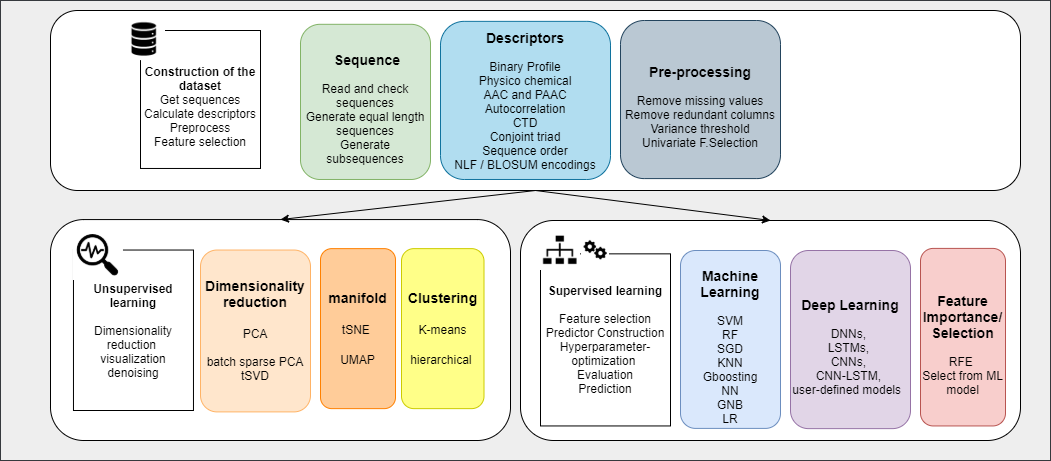
\includegraphics[width=\linewidth]{propythia_workflow}
    \caption{Schematic representation of the modules in ProPythia~\cite{Sequeira2020ProPythia:Learning}.}
    \label{fig:propythia_workflow}
\end{figure}

The first main objective of this study regarding \textit{ProPythia} was to extend its calculation of descriptors to also include \gls{DNA} descriptors. To accomplish this, a module (similar to the one for proteins) was developed that can be imported by other modules to create a \textit{Python} dictionary containing all calculated descriptors. As the remaining \gls{ML} steps are independent of one another, \textit{ProPythia} is now capable of performing the whole \gls{ML} pipeline for \gls{DNA} data. The list of implemented \gls{DNA} descriptors can be found later in section~\ref{cha:descriptors}.

The other key objective was the development of a complete \gls{DL} pipeline for the classification of \gls{DNA} sequences. Although \textit{ProPythia} already includes a module for \gls{DL}-based classification, it was not used to complete this step since it was not built in \textit{PyTorch}, but rather in \textit{Tensorflow/Keras}. The implemented \gls{DL} steps were encoding, data processing, model building and training, model evaluation, and, finally, hyperparameter tuning. 

These \gls{DL} steps, along with the calculation of descriptors, were built as separate and independent modules that can be used in combination with other modules, including those developed now and those already present in \textit{ProPythia}. For example, it is possible to use the new \gls{DNA} encodings to train a \textit{ProPythia}'s \gls{DL} model and also use \textit{ProPythia}'s protein encoders to train a \gls{DL} \textit{PyTorch} model. Similarly, it is also possible to use the \gls{DNA} descriptors to train a \textit{ProPythia}'s shallow \gls{ML} model and also use \textit{ProPythia}'s protein descriptors to train a shallow \gls{ML} \textit{PyTorch} model.

Figure~\ref{fig:meu} provides an overview of the developed workflow.

\begin{figure}[htbp]
    \centering
    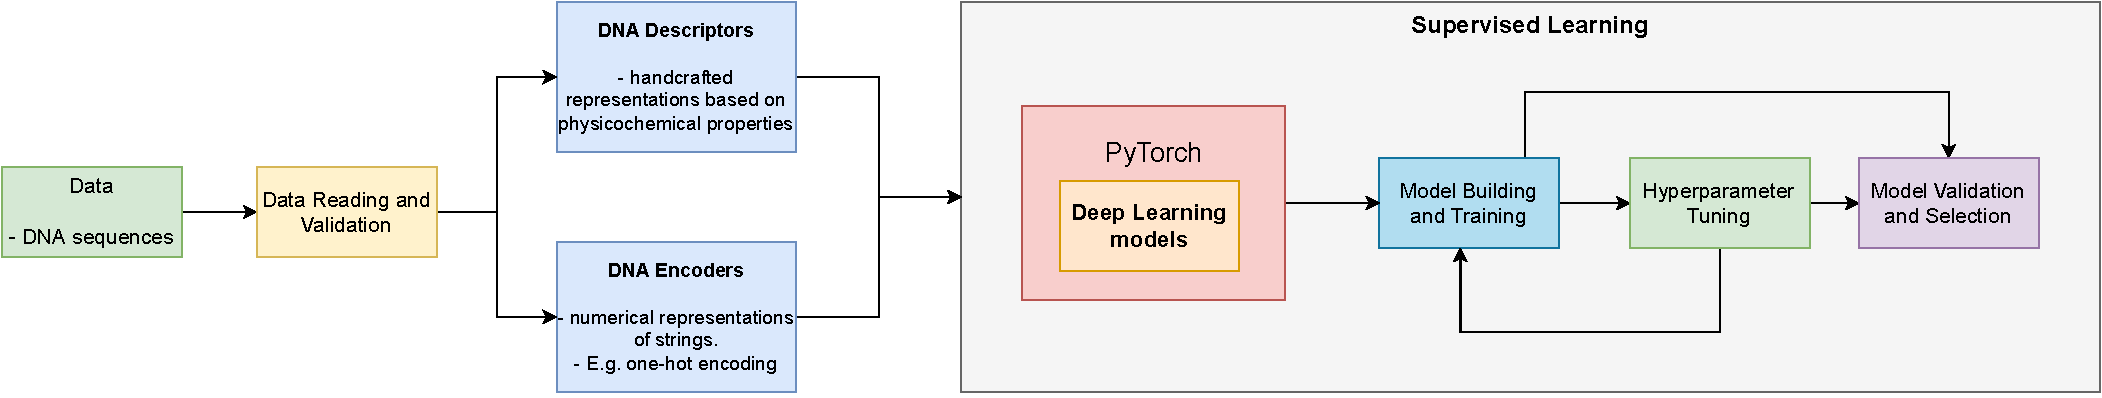
\includegraphics[width=\linewidth]{meu}
    \caption{Implemented workflow in ProPythia for Deep Learning DNA classifications.}
    \label{fig:meu}
\end{figure}

Figure~\ref{fig:integration_propythia} provides a visualization of how the implemented modules of \gls{DL} \gls{DNA} classification is integrated in \textit{Propythia}. The coloured modules were the new ones implemented and the gray ones are from \textit{ProPythia}.

\begin{figure}[htbp]
    \centering
    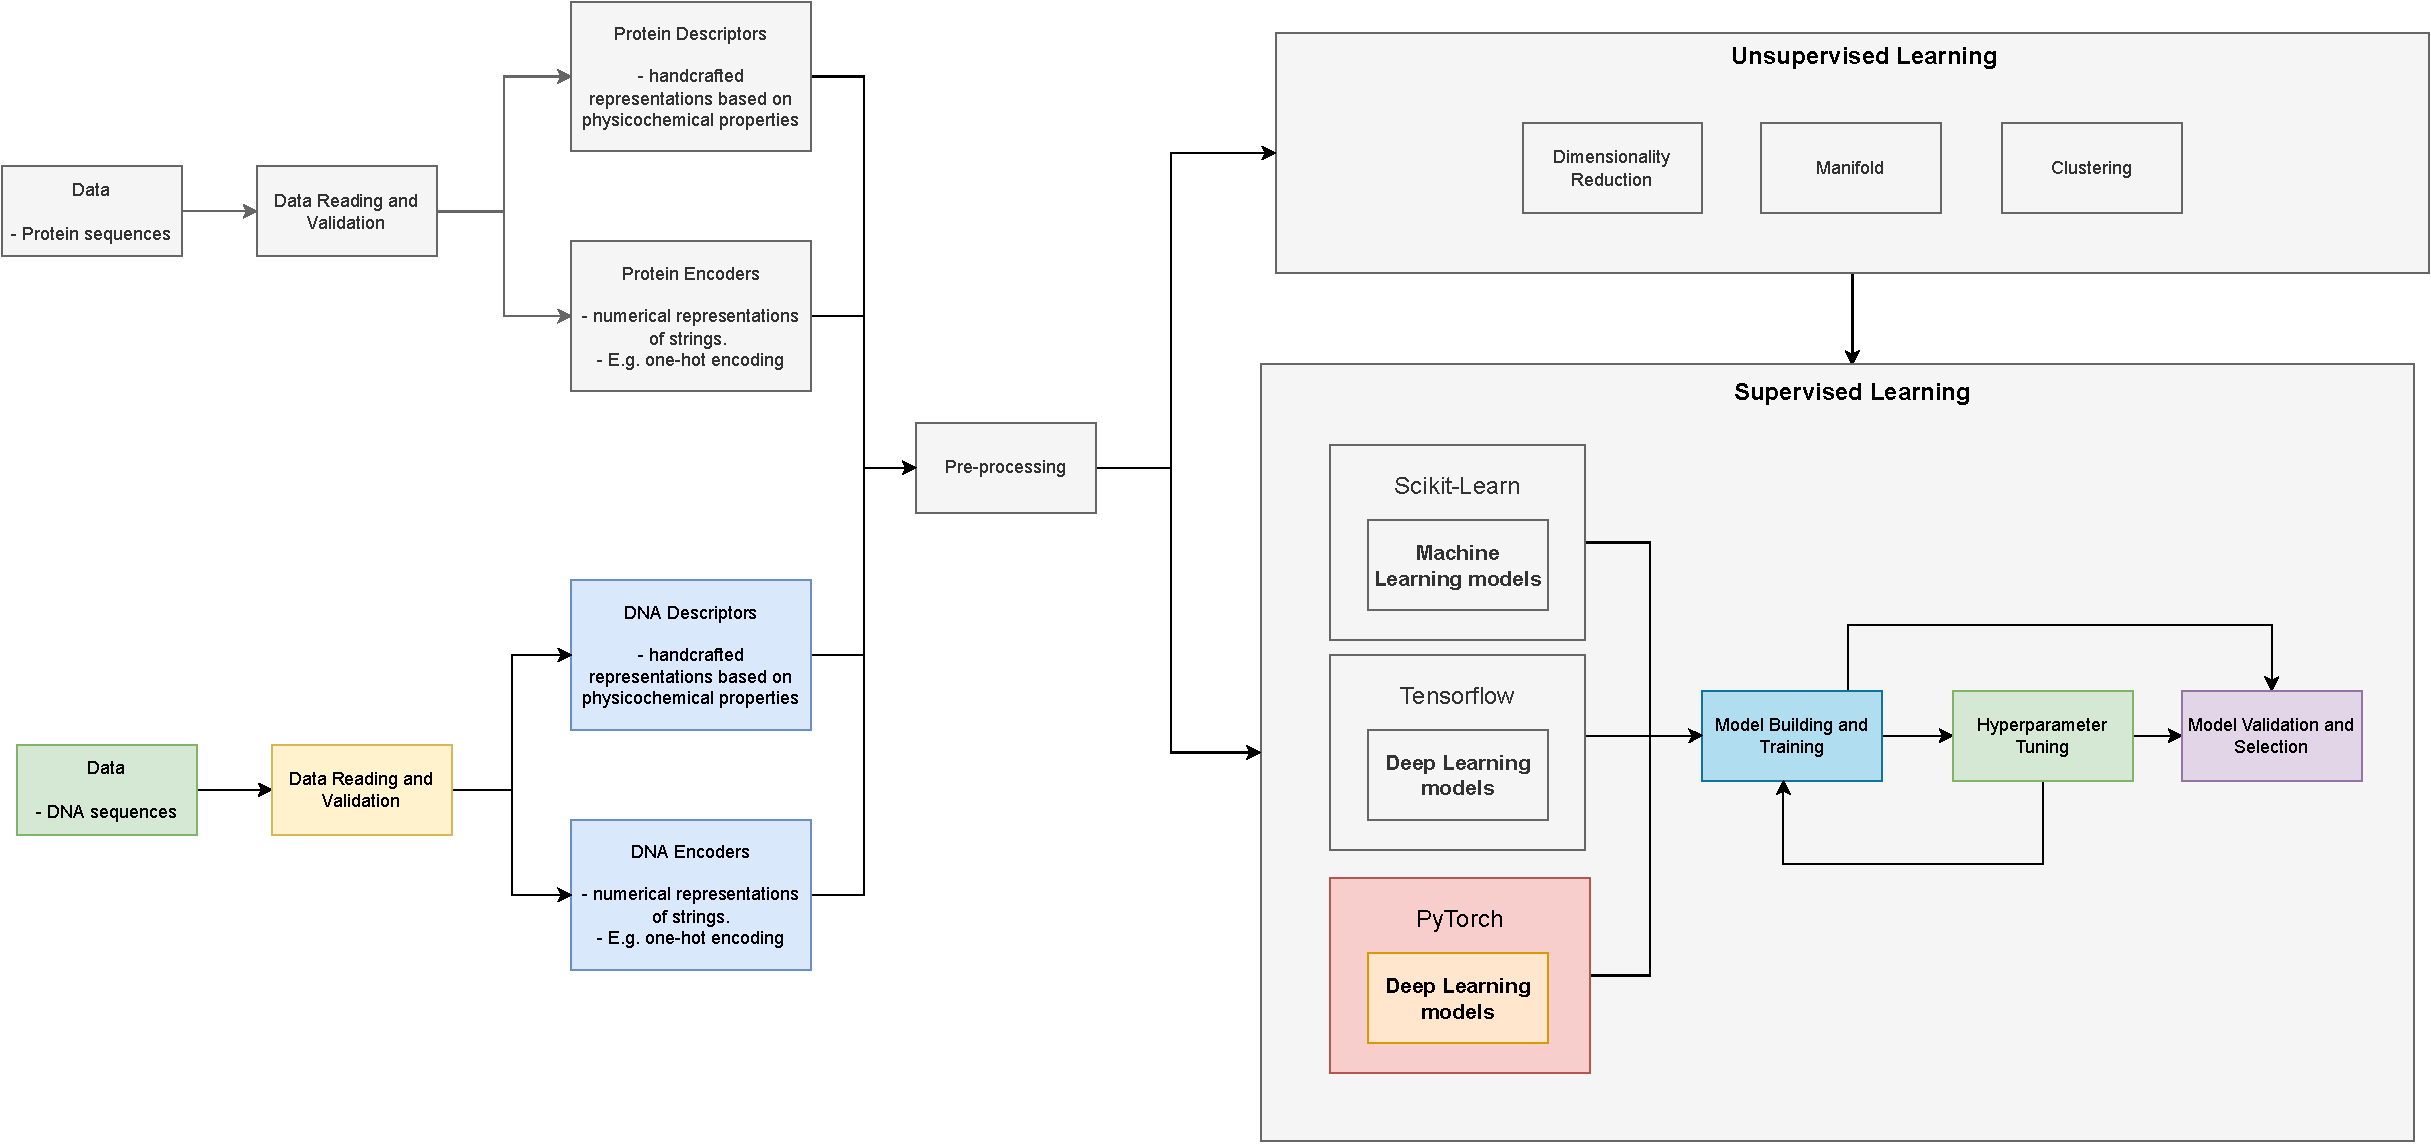
\includegraphics[width=\linewidth]{integration_propythia}
    \caption{Integration of implemented modules in ProPythia.}
    \label{fig:integration_propythia}
\end{figure}

Both implementations of \gls{DNA} descriptors and the \gls{DL} pipeline had a step in common: the data reading process. As a result, a data reading module was developed to read \gls{DNA} sequences from \textit{CSV} or \textit{FASTA} files. The data is then validated, which means that every letter in the sequence has to be either an \gls{A}, \gls{C}, \gls{G}, or \gls{T}.

\section{OMNIA}

\textit{OMNIA} is the \gls{AutoML} platform for bioinformatics of \textit{OmniumAI}. It contains a set of methods for the analysis of biological data. Currently, it offers tools for analyzing the data in the following categories - compounds, proteins, metabolomics, transcriptomics, single-cell transcriptomics and text mining. An overview of this platform is depicted in Figure~\ref{fig:omnia_before}.

\begin{figure}[htbp]
    \centering
    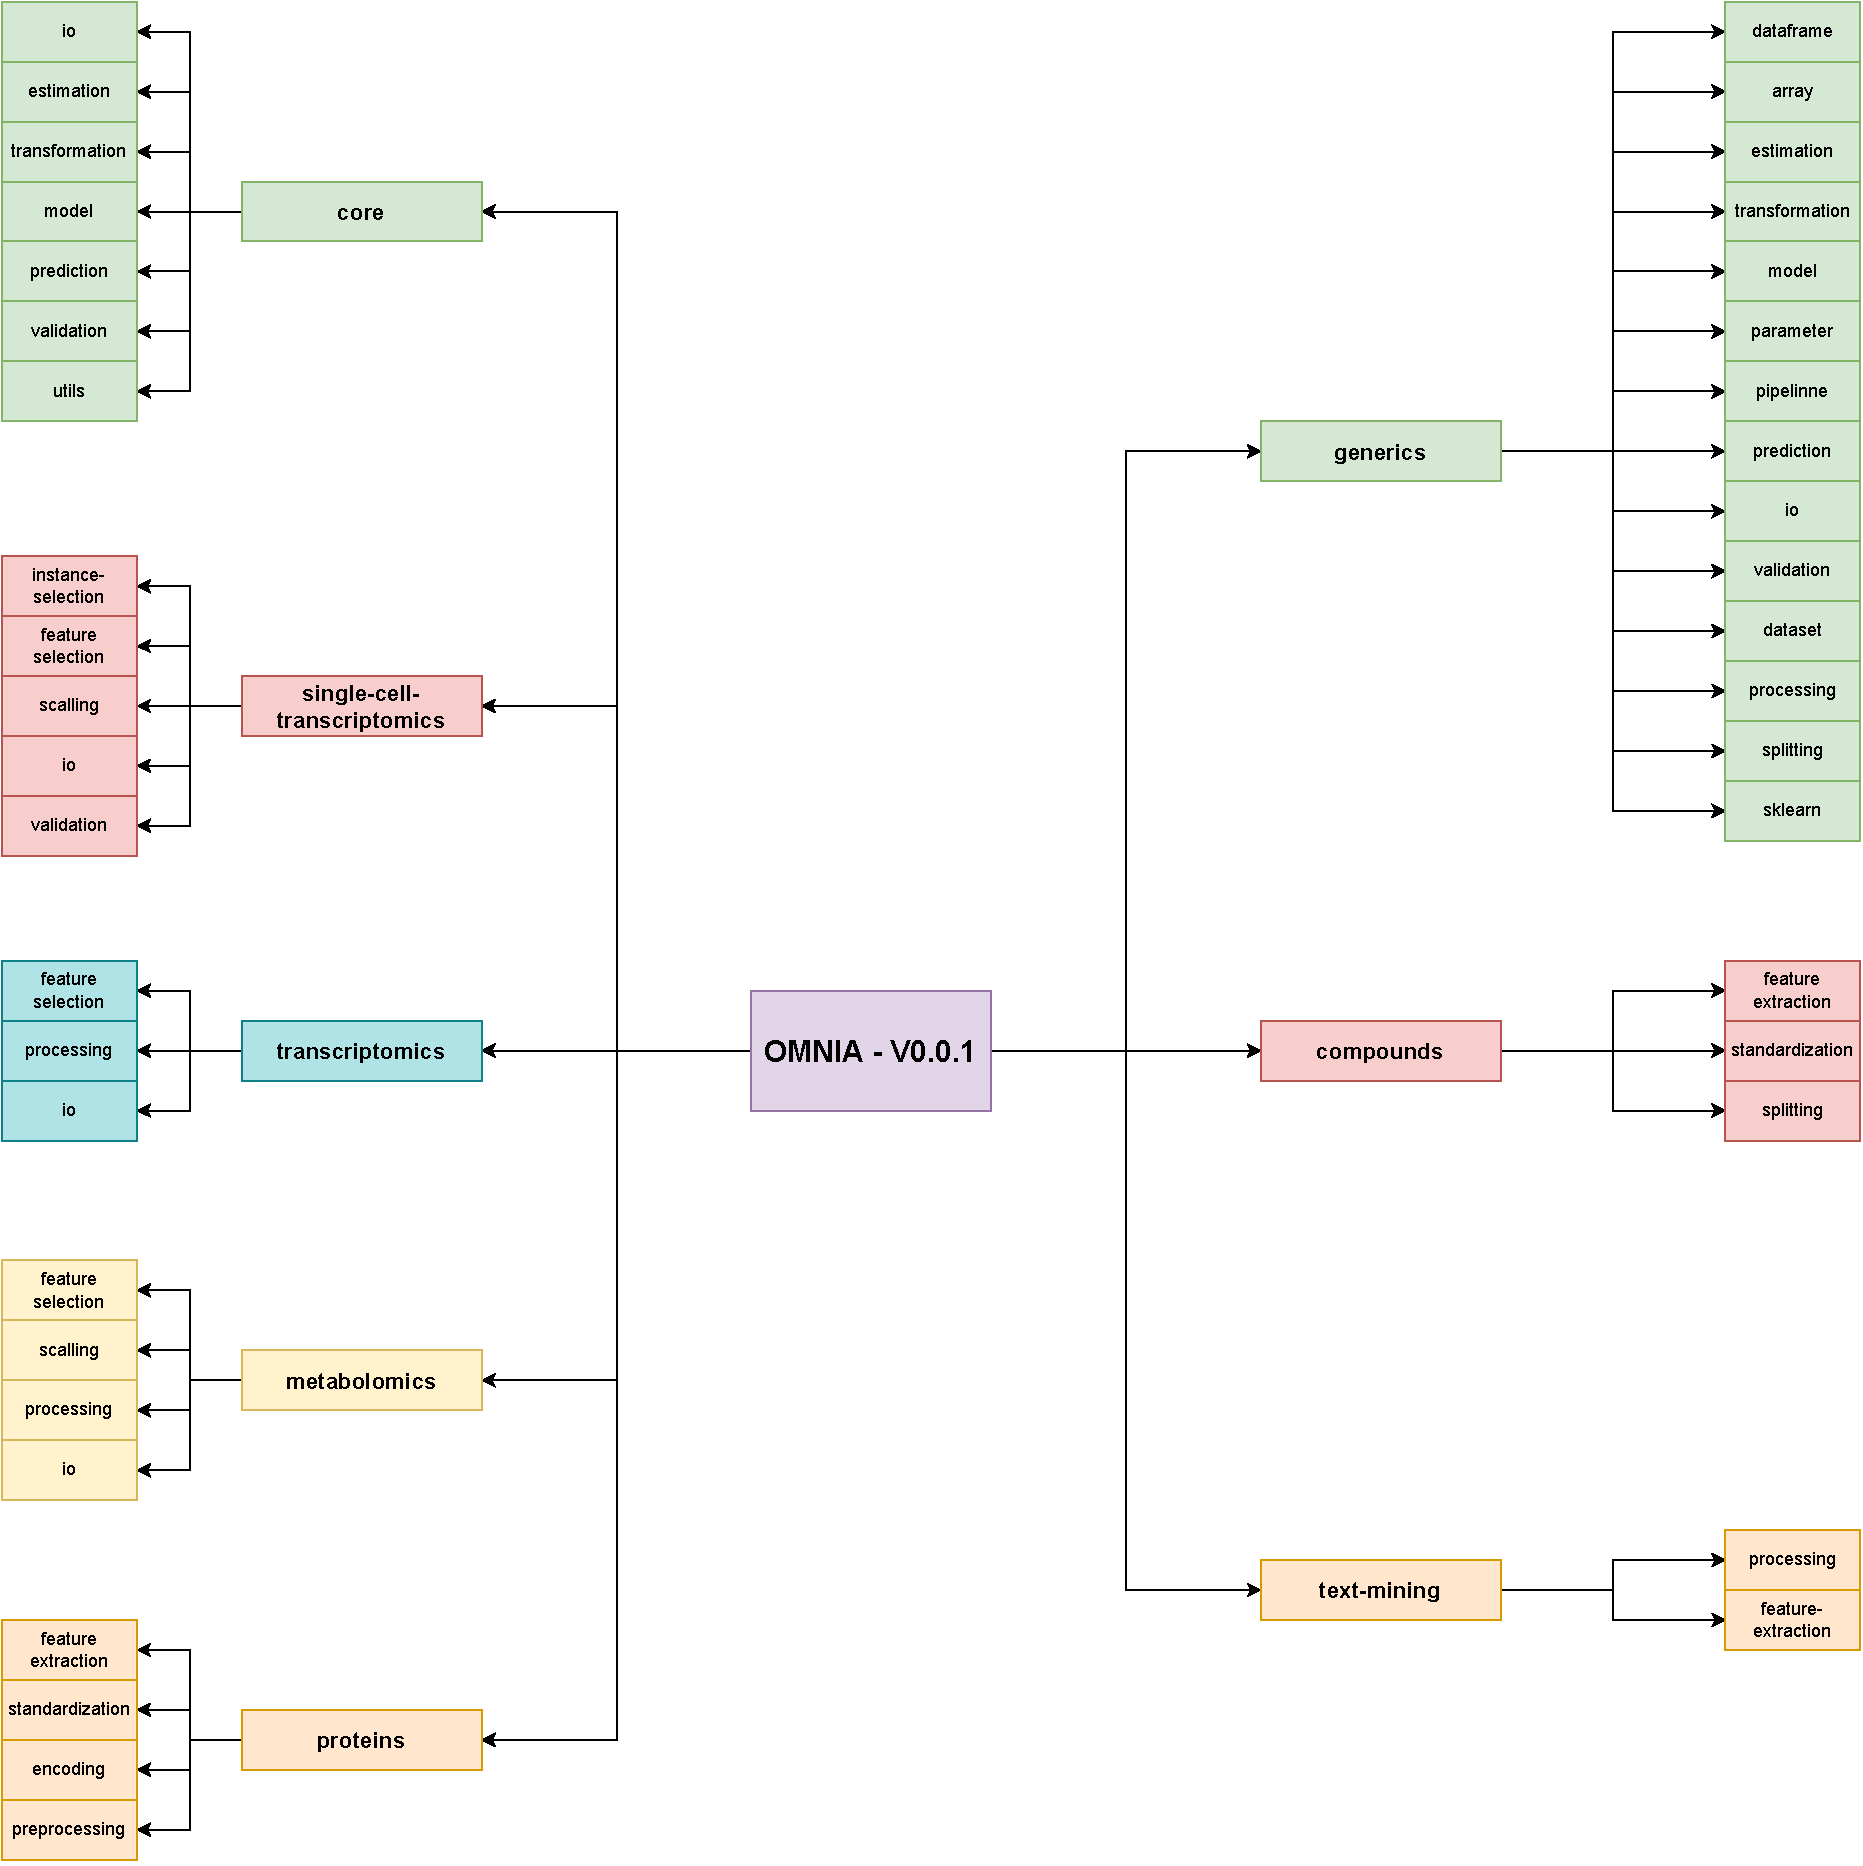
\includegraphics[width=0.7\linewidth]{omnia_before}
    \caption{OMNIA overview before implementations.}
    \label{fig:omnia_before}
\end{figure}

As it can been observed in Figure~\ref{fig:omnia_before}, there are two modules on the left called \textit{generics} and \textit{core}. These are the fundamental pillars that provide structure for the whole project. The generics module contains generic objects, such as dataframe, estimator, and model, that may be used by other packages and are built using Sklearn\footnote{https://scikit-learn.org/stable/} and Autogluon\footnote{https://auto.gluon.ai/stable/index.html} libraries. Then, for the \textit{core} module, the idea was for it to include the interfaces and some basic and generic implementations that have no external dependencies. And after that, further generic implementations with external dependencies would be in \textit{generics}. At the moment, the only feature the \textit{core} has are the interfaces. The remaining generic and base implementations are in \textit{generics} since they almost always rely on Sklearn or Autogluon. In fact, \textit{core} module will probably be removed from OMNIA.

The first main objective in \textit{OMNIA} was similar to the \textit{ProPythia}'s one, which was the creation of a module that calculates \gls{DNA} descriptors. This module would serve the same purpose of the previously mentioned ones (proteins, metabolomics, etc), which is a tool to process, in this case, \gls{DNA} sequences. The implementation from \textit{ProPythia} was re-utilized, but adapted to the \textit{OMNIA} requirements and dependencies.

Then, the other key objective was the addition of \gls{DL} \textit{PyTorch} models, as well as the functions that allow the \textit{OMNIA} to use them. These functions include train, test, validation and data related processes, which were also implemented with \textit{PyTorch}. Both the models and the functions would be developed in the \textit{generics} module as it is expected that they will be used in all the other modules that handle different types of biological data, such as proteins, metabolomics, etc. Identical to the previous objective, the \textit{PyTorch} models and functions were re-utilized from \textit{ProPythia}, but adapted to the \textit{OMNIA} requirements and dependencies.

Figure~\ref{fig:done-in-omnia} illustrates how the \textit{OMNIA} platform incorporates both of these goals. It is also possible to see the models that were already implemented and how the new ones integrate among them in the \textit{generics} module.

\begin{figure}[htbp]
    \centering
    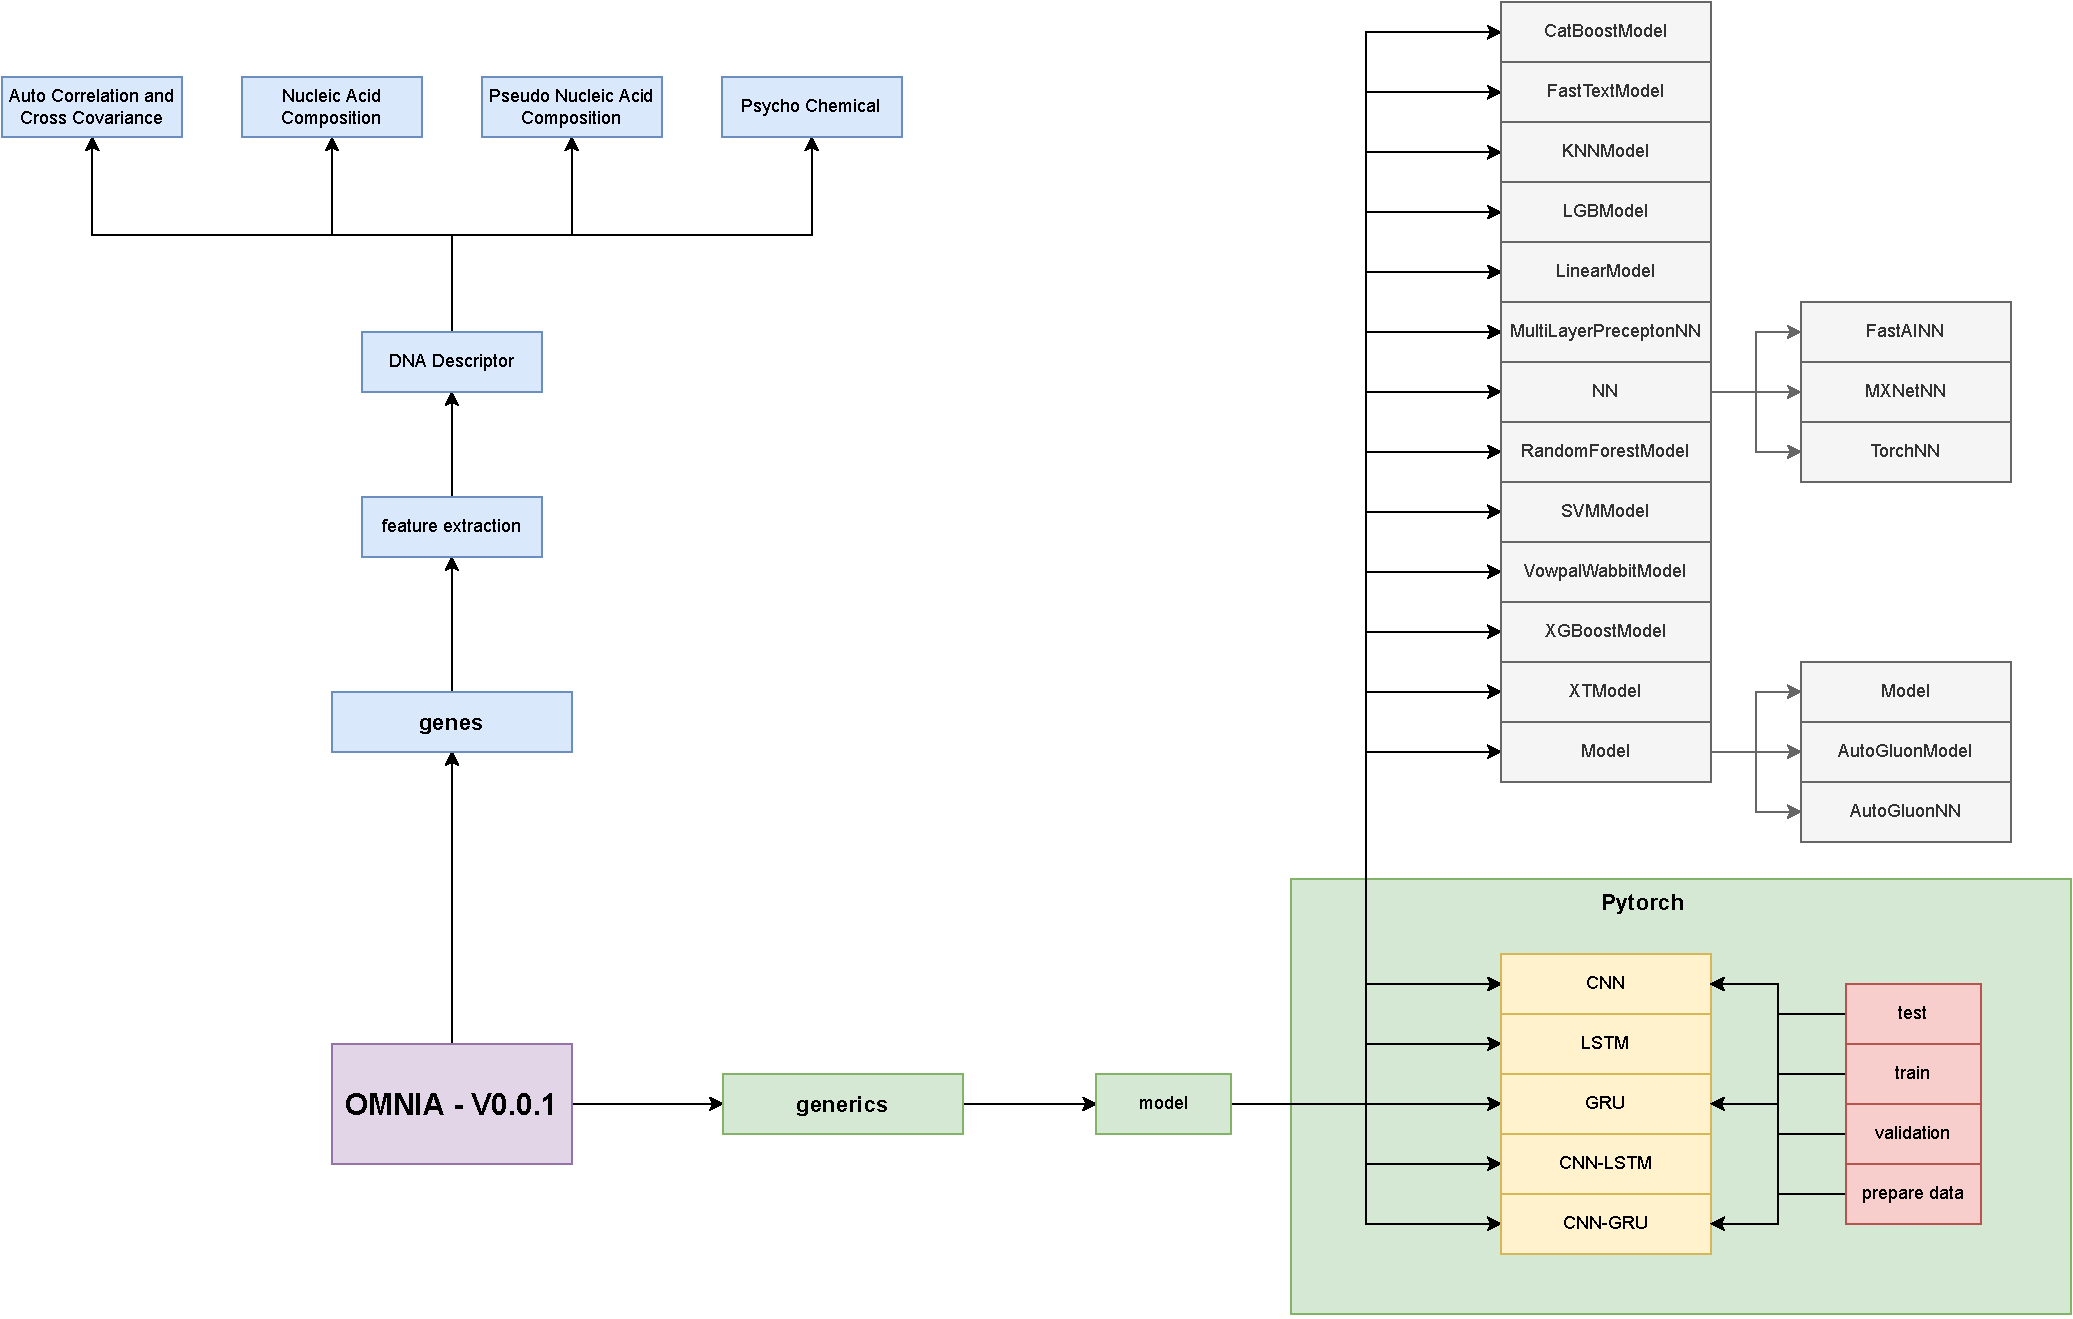
\includegraphics[width=\linewidth]{done-in-omnia}
    \caption{Modules integration in OMNIA.}
    \label{fig:done-in-omnia}
\end{figure}

Then, figure~\ref{fig:omnia-integration} provides the overview of the entire platform, highlighting the implemented modules and how they integrate in OMNIA. In a nutshell, the \textit{generics} module was extended to include \gls{DL} \textit{PyTorch} classifications, and an independent biological data processing was added, the \textit{genes} module, that provides the calculation of \gls{DNA} descriptors.

\begin{figure}[htbp]
    \centering
    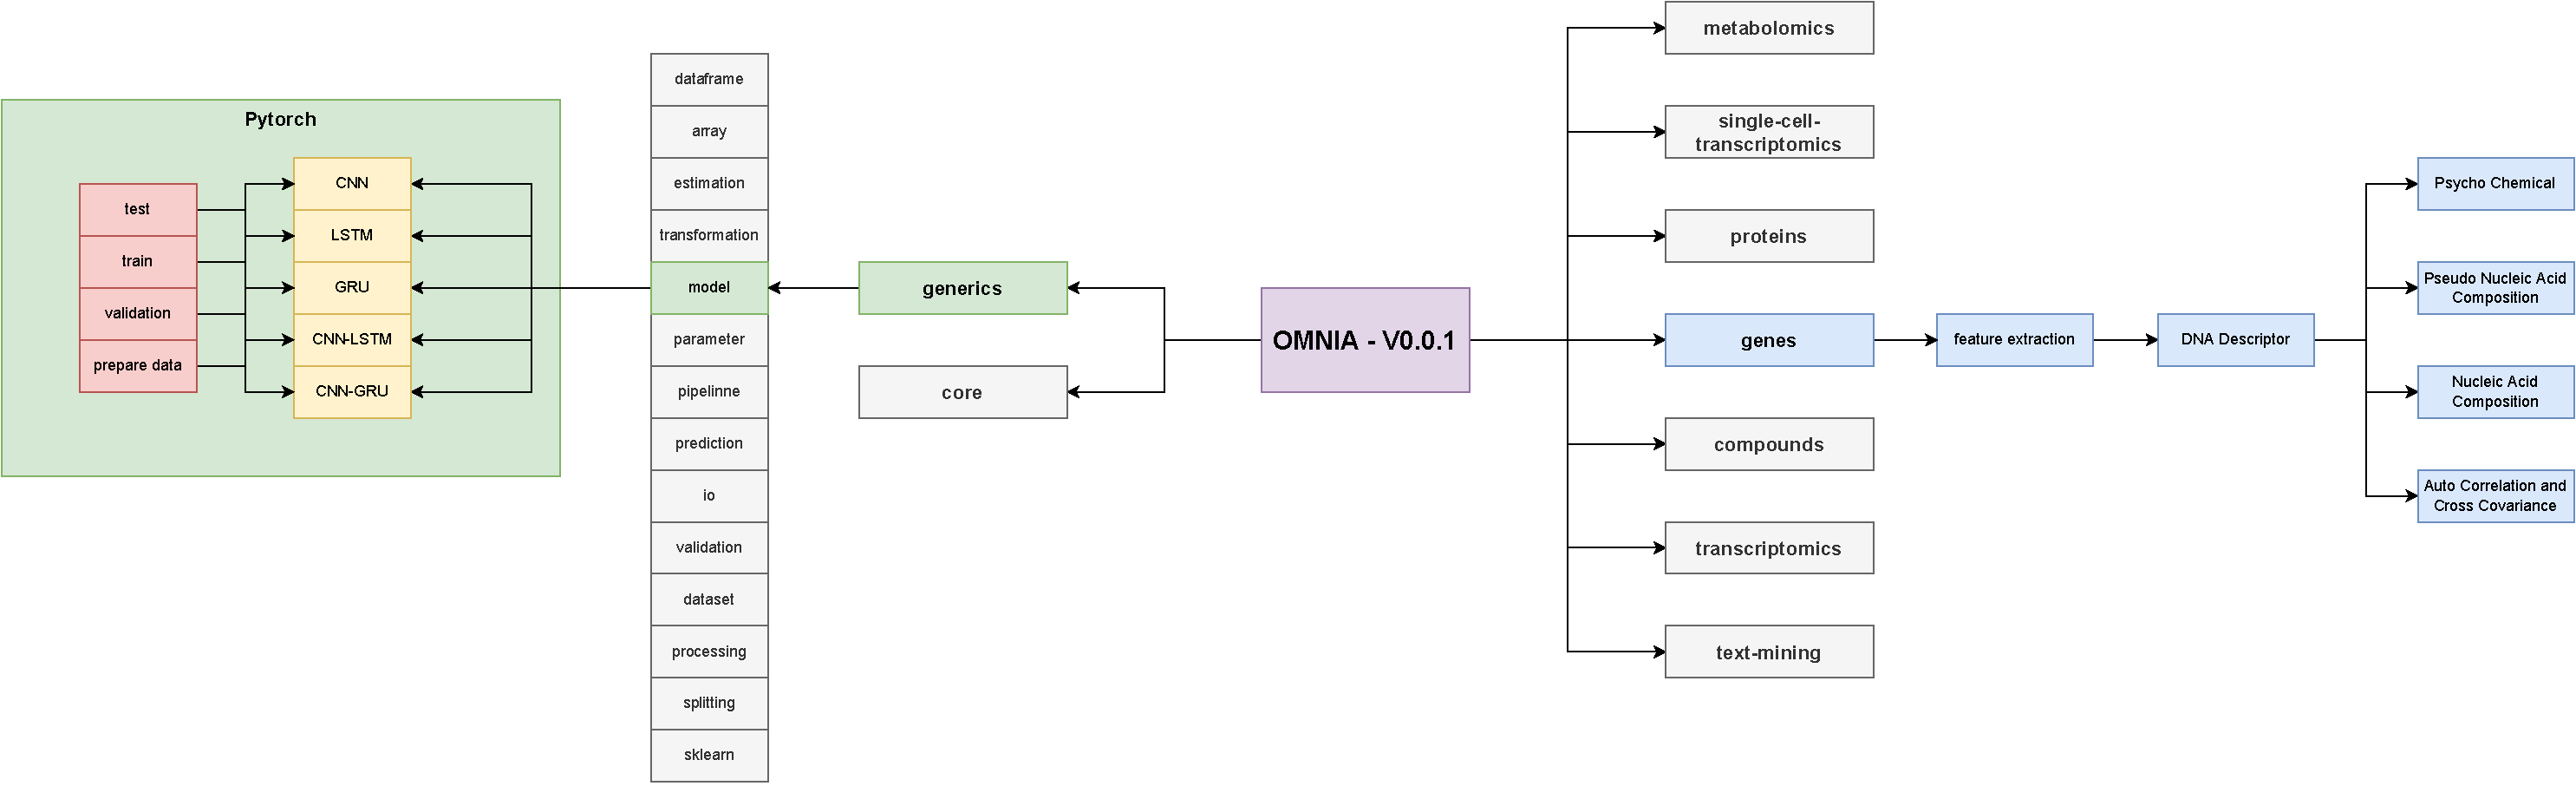
\includegraphics[width=\linewidth]{omnia-integration}
    \caption{OMNIA overview after implementations.}
    \label{fig:omnia-integration}
\end{figure}

Similar to \textit{ProPythia}, it is expected that the \gls{DNA} descriptors and \gls{DL} models will be used in combination with other models and biological data handling modules. For example, it is possible to use the \gls{DNA} descriptors to train an \textit{OMNIA}'s shallow \gls{ML} model and also use the descriptors from \textit{proteins} module to train a shallow \gls{ML} \textit{PyTorch} model. Likewise, it is also possible to use the \gls{DNA} encoders to train a \textit{OMNIA}'s \gls{DL} model and also use the encoders from the \textit{proteins} module to train a \gls{DL} \textit{PyTorch} model.